\documentclass[pageno]{jpaper}
%\documentclass[sigconf,screen]{acmart}
\usepackage[pdf]{graphviz}
\usepackage{pgf-umlsd}
\usepackage{listings}
\usepackage{enumitem}
\usepackage{amsfonts}
\graphicspath{ {./figs/} }
\usepackage{framed,color,verbatim}
\usepackage{mathtools}
\usepackage{flushend}
\definecolor{shadecolor}{rgb}{.9, .9, .9}

\newenvironment{code}%
   {\snugshade\verbatim}%
   {\endverbatim\endsnugshade}

%replace XXX with the submission number you are given from the ASPLOS submission site.
\newcommand{\asplossubmissionnumber}{XXX}

\usepackage[normalem]{ulem}

\begin{document}

\title{A ZK-Based Multi-Blockchain Communication Protocol for Minimal Trust Base}
%\author{Sinka Gao, Guoqiang Li, Hongfei Fu , Heng Zhang}
\newcommand{\dprotocol}{ZK Multi-Chain Aggregator }
\date{}
\maketitle
\thispagestyle{empty}
\begin{abstract}
%\dprotocol is a universal firmware that synchronizes states between different smart contracts on different blockchains. 
In the realm of blockchains, synchronization challenges are two-folded. First, contracts from different blockchains can not communicate with each other which makes it hard to establish a trustworthy communication channel for them to share and maintain a universal state between each other. Second, transactions on different blockchains can hardly be ordered thus interference is common and we need a novel way to avoid and handle interference. Traditional solutions which involve third parties have safety and liveness issues and thus need to compromise between safety, permissionless, and liveness.  \dprotocol is a multi-blockchain execution layer that leverages the power of zero-knowledge proof to minimize the trust base of multi-chain communication which does not compromise on safety, liveness, permissionless, and atomicity. In contrast to traditional blockchain bridges which perform transactions on different blockchain separately and uses a relay system to enforce the order of transactions and prevent interference, \dprotocol uses a completely new approach. For each multi-chain transaction, \dprotocol simulates the multi-chain transactions in its aggregator chain and uses zero-knowledge proofs of the simulation to convince involved blockchains to update their local state accordingly.  On top of this layer, rich applications over multi-blockchains can run safely and efficiently.
\end{abstract}

\section{Introduction}
As an emerging distributed computing paradigm, blockchain is rapidly evolving in areas such as digital finance and cryptography. Existing blockchain projects adopt different blockchain architectures and protocols and, as a consequence, it is generally difficult for different blockchain systems to flow information to each other. Thus, different blockchains themselves are born isolated islands which brought limitations to the overall usability, functionality, and scalability of blockchain technology~\cite{anati2013innovative}.

\subsection{The Problem}
In general, the difficult part of cross-chain communication is that there is no proper way for a blockchain transaction to query the state of another blockchain. This is because a blockchain system is a decentralized computing system that contains a large set of nodes connected over a peer-to-peer network and a successful transaction needs to be audited on multiple nodes, which means that a transaction's result can only depend on the blockchain's internal states otherwise the result of a transaction will be inconsistent between different auditing nodes. 

As an example, we take a look at the cross-chain decentralized exchange~\cite{zetzsche2020decentralized} which is a typical scenario of multi-chain communication. In such a scenario, suppose that Alice would like to swap one token from Bob on blockchain $C_A$ by spending one token on blockchain $C_B$, then it follows that we need at least two transactions $tx_A$ (Alice gets a token from Bob on blockchain $C_A$) and $tx_B$ (Alice pays a token to Bob on blockchain $C_B$) to be executed atomically.

Moreover $tx_A$ and $tx_B$ need to be executed in a safe manner that either both of them succeed or both fail. If it is not the case, then either Alice loses a token on blockchain $C_B$ or Bob loses a token on blockchain $C_A$. However since $tx_A$ cannot access any info of $tx_B$, a protocol needs to be designed to achieve a safe swap.

%Recently, the growing demand for flowing value between different chains stimulates the demand for secure and consistent cross-chain exchange protocols for cross-chain communication and bookkeeping.  To address the safety, liveness, permissionless, and linearizability problem of various protocols, and to build trustworthy consensus between different blockchain networks, cross-chain techniques received a lot of attention.

To address the synchronization problem, many protocols are developed in the literature including time hash lock \cite{poon2016bitcoin}, interledger’s stream protocol \cite{zhang2021enabling}, relay system \cite{lys2021r}, SPV \cite{nakamoto2008bitcoin}, side chain\cite{singh2020sidechain,deng2018sidechain}, side chain with ZKP (zero-knowledge proof) \cite{sidechainzkp}, and most of them introduce relayers \cite{sun2020collaborative-relay, warren20170x-relay} to establish an information channel from source block chain A to target block chain B as in figure \ref{relayer-connection}:
\begin{figure}[!ht]
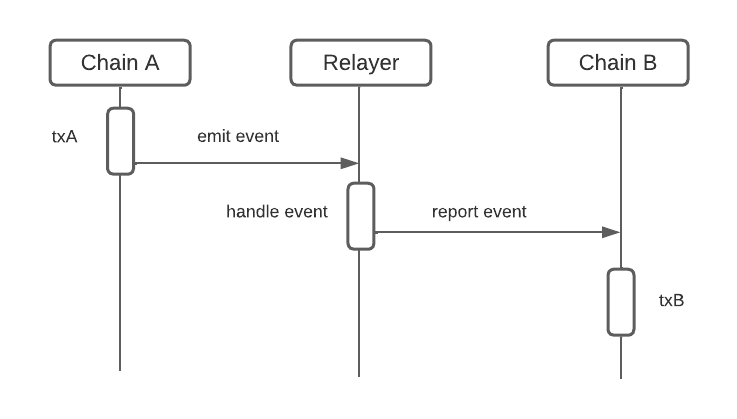
\includegraphics[scale=0.6]{relayer}
\caption{Forwarding message using a relayer}
\label{relayer-connection}
\end{figure}

\subsection{Technical Challenges}
The major security challenge regarding the module in Figure \ref{relayer-connection} is that we require the relayer to be honest and authorized. A centralized relayer can be built such that chain B only accepts information reported from a trusted relayer. In such a solution, safety is enforced since the trusted relayer signs all their messages with their private key and $tx_B$ in chain B checks the signature accordingly. However with such a centralized setup, the relayer becomes one of the most important trust bases for the protocol to work which may lead to SIOF (single point of failure) if the relayer is hacked or misbehaved.

%This built-in drawback of blockchains makes it hard to execute a group of transactions involving different chains so that either all of them or none of them succeed on different chains. 

To take a step further, we consider two bundled transactions $T_1$ and $T_2$. $T_1$ contains $tx_A^1$ on blockchain $C_A$ and $tx_B^1$ on blockchain $C_B$. $T_2$ contains $tx^2_C$ on blockchain $C_C$ and $tx_B^1$ on blockchain $C_B$. Then it follows that the safety property requires transactions in $T_1$ and $T_2$ both succeed or none of them succeed. In such senario, the safety of relayer does not enforce the safety of the bundled transactions as there might be interference between the execution of $T_1$ and $T_2$ (e.g. the execution sequence is $tx_A^1$, $tx_C^2$, $tx_B^1$, $tx_B^2$). 

Suppose that a protocol is designed to help carry out such bundled transactions between blockchains, then we can define the safety, permissionless, liveness, and linearizability properties of the protocol as follows:

\smallskip\noindent\emph{Permissionless.} Any nodes of a certain blockchain are allowed to join the communication network.

\smallskip\noindent\emph{Safety.} All state updates for a single transaction are either successful or fail on all involved blockchains.

\smallskip\noindent\emph{Liveness.} All valid transactions will eventually succeed on all blockchains.

\smallskip\noindent\emph{Linearizability.} All concurrent successful transactions are always linearizable so that the consequent state of a group of concurrent transactions $tx_i$ is equivalent to performing the transactions sequentially in a special order that respects the happen-before relation of the original order.

Although various solutions tried to tackle the above problems, they usually restricted the scope of use-cases to be transactions within two blockchains where the atomicity and liveness properties is simpler comparing to multi-chain scenarios.

Recently the development of PCS (Polynomial Commitment schemes \cite{boneh2020halo-pcs,boneh2020efficient-pcs,kate2010polynomial-pcs}) provides a new way to convince others that the polynomial has certain evaluation at certain point without redo the calculation. Based on this technique, ZKSNARK (Zero-Knowledge Succinct Non-Interactive Argument of Knowledge \cite{petkus2019and, groth2016size-scheme,chiesa2020marlin-scheme, gong2022analysis-scheme, setty2020spartan-scheme, fiore2016security-scheme}) become technically mature which is often used to prove that a statement is true, without revealing any information beyond the validity of the statement itself. Some usage of ZKSNARK in cross-chain communication can be found in \cite{sidechainzkp, cao2020-zk-atomic, garoffolo2020zendoo} which mainly focus on communications between two blockchains by providing a secure (ZKP backed) relayer.

\subsection{Our Contribution}

In this paper, we make the following contributions:
\begin{itemize}
\item We consider the general case of multi-chain bundled transactions and provide a novel way to preserve the linearizability of transactions cross multiple blockchains. In particular, instead of executing multiple transactions on different blockchains and using relayers to synchronize them, we simulate the transactions on our aggregation layer and generate ZKP (zero-knowledge-proofs) to convince involved blockchains to update their state accordingly afterwards. 

\item Our approach not only enforces linearizability natually, but also allows transaction to be designed to have a view of multichain states. For example, if a traditional two-chain transaction contains $t_1$ and $t_2$ then $t_1$ can only see the state on blockchain $C_1$ and $t_2$ can only see the state of blockchain $C_2$. By using our approach, $t_1$ and $t_2$ can both see the global state of $C_1 \times C_2$.

\item We provide a permissionless solution by encoding the consensus algorithm into ZKP. By doing so we get the following benefits.
\begin{itemize}
    \item Compares to other solutions which requires the upper bound number of monitors are fixed, our solution allows new anonymous nodes to register them-self into the system. We believe that only by providing a dynamic system, the liveness property is then enforced.
    \item We allow user to trigger bundled transactions not only on native blockchain but also on our aggregator chain which was technically hard as we need to prevent dishonest nodes that systemically ignore transactions triggered on aggregator chain.
    \end{itemize}
\end{itemize}
\section{Preliminaries}
\label{prelimiary}
While there are many existing protocols designed for specific scenarios and they focus on preserving different properties with various trust base. \dprotocol targets to achieve liveness, safety, permissionless, and linearizability properties by using zero-knowledge proof to provide a universal layer that synchronizes states between different smart contracts on different blockchains, and this layer together with its communication protocol can be used as a multi-chain communication framework. Below we first briefly review several key concepts in our protocol and then describe the main idea behind \dprotocol. For a detailed description of these concepts, we refer to \cite{robinson2021survey}. 

\smallskip\noindent\textbf{Blockchain.}
A blockchain is a distributed database that is shared among a network of distributed nodes \cite{chen2018survey}. As a database, transactions are first submitted and organized in blocks, while each block is a data structure that records the most recent transactions which are not yet validated. Once a block was validated the state of the whole distributed database is updated accordingly.

\smallskip\noindent\textbf{Bundled multi-chain Transaction.}
We use $C$ (with possible subscripts) to denote a particular blockchain system with distributed nodes. For a blockchain $C_k$ indexed with $k$, We use $S_k$ to denote the whole state of a blockchain $C_{k}$ and $s_k$ to describe a \emph{partial} state in $S_k$.

Given a group of blockchains $C_{1}, C_{2}, \cdots, C_{k}$, we say a transaction $tx$ is a bundled multi-chain transaction if it is composed of a sequence of transactions $tx_{k_0}^0$, $tx_{k_1}^1$, $\cdots$ $tx_{k_j}^j$ such that the $j$th involved sub-transaction $tx_{k_j}^j$ is supposed to be executed on $C_{k_j}$ locally and the behavior of each $tx_{k_j}^{j}$ depends on state $s_{k_j}$. 

In a bundled transaction $tx$, We use $s= \langle s_1, s_2, \cdots, s_k \rangle$ to denote the underlying global state of $tx$ where $s_k$ denotes the projection of $s$ on the blockchain $C_k$. Moreover each local transaction $tx_k^j$ is executed on the partial state of $s_k$ in $C_k$. For example, a bundled transaction could look like the following. 
\begin{lstlisting}[escapeinside={(*}{*)}, backgroundcolor = \color{lightgray}, basicstyle=\small,]
tx(s) {
    (*$s^1 = \langle tx_0(s_0^0), s_1^0, s_2^0, \cdots \rangle$*)
    (*$s^2 = \langle s_0^1, tx_1(s_1^1), s_2^1, \cdots \rangle$*)
    ....
    (*$s^n = \langle s_0^{n-1}, s_1^{n-1}, s_2^{n-1}, tx_n(s_{k}^{n-1})\rangle$*)
}
\end{lstlisting}
where $tx_0$ is performed on local state $s_0$, $tx_1$ is performed on local state $s_1$ ..., and the global state $s$ is changed to $s^n$ after $tx$ is fully performed.

\smallskip\noindent\textbf{Aggregator Chain.}
In this work, we will introduce an extra blockchain to store the global state $s$. We denote this chain as an \emph{aggregator chain} to distinguish it from other blockchains $C_{k}$ involved in a bundled multi-chain transaction $tx$. Moreover, we call the other blockchains \emph{native chains}.

\smallskip\noindent\textbf{Merkle Tree Encoding of a Global State.}
Merkle tree \cite{becker2008merkle} is a tree (see Figure \ref{merkle-tree}) in which every leaf node is labeled with the cryptographic hash (P = hash(leaves)) of a data block, and every non-leaf node is labeled with the cryptographic hash of the labels of its child nodes. Each data block has a unique Merkle tree index (MTI) and each MTI encodes a unique path from top to leaf.\\

\begin{figure}[!ht]
\centerline{
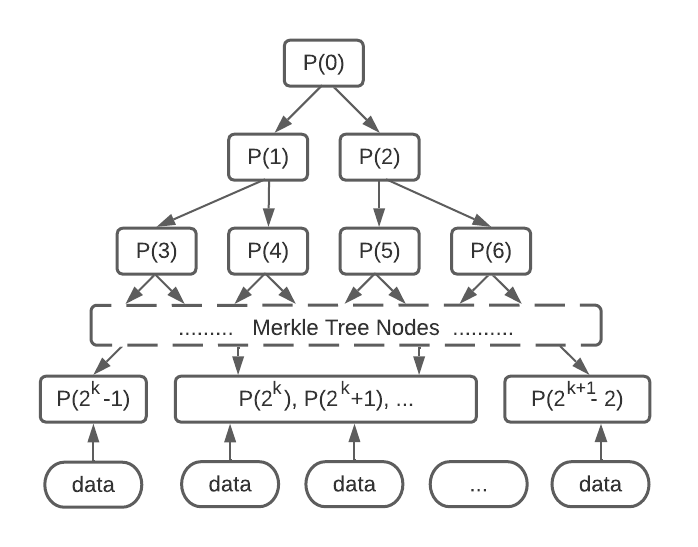
\includegraphics[scale=0.6]{merkle-tree}}
\caption{Merkle tree structure}\label{merkle-tree}
\end{figure}

\smallskip\noindent\textbf{State Pinning.}
State Pinning \cite {robinson2019anonymous} is defined as including the state of one blockchain in another blockchain. In our scenario, we encode our global state into the Merkle tree and use the Merkle root hash to pin the global state in native blockchains to ensure that the global state used in the simulation of transactions is consistent.

\smallskip\noindent\textbf{Side Effect.}
We denote the changes of $tx_i^k$ on chain-state $C_k$ other than the partial state $s_k$ to be the side effect $e_k$ of of $tx_i^k$. Side effects can be emitting events on native chains or native chain contract calls.

\smallskip\noindent\textbf{Polynomial Commitment schemes.}
Polynomial commitment schemes (PCS) \cite{boneh2020halo-pcs,boneh2020efficient-pcs,kate2010polynomial-pcs}, provides the ability to commit to a polynomial over a finite field and prove its evaluation at points. A succinct PCS has commitment and evaluation proof size sublinear in the degree of the polynomial. An efficient PCS has sublinear proof verification. Any efficient and succinct PCS can be used to construct a SNARK \cite{mayer2016zk} with similar security and efficiency characteristics.

\smallskip\noindent\textbf{Zero Knowledge Proof of Program Execution}
Since PCS provides a scheme to prove the evaluation of polynomials at certain points, we can convert program evaluation into polynomials equations so that the problem of proving a program has certain results can be converted into problems of polynomial equations. Furthermore, a zero-knowledge proof \cite{cramer1998zero-zkp,kate2010constant-zkp,damgaard1998commitment-zkp} of program execution is a PCS proof that can be used by a prover to convince a verifier that a program is executed correctly without leaking any private information.

\dprotocol derives the basic ideas from multi-way sidechain (multiple blockchains with a shared sidechain) and solves the trustworthy problem of the third parties by verifying the computation from the sidechain via ZKSNARK proofs. In \dprotocol, we denote our specific sidechain as an aggregator chain and involved blockchains of bundled transactions as native chains.\\
\newline
More precisely, instead of executing transactions in a special order in a bunch of native blockchains, we do the following (see figure \ref{main-idea}):

\begin{figure}[!ht]
\centerline{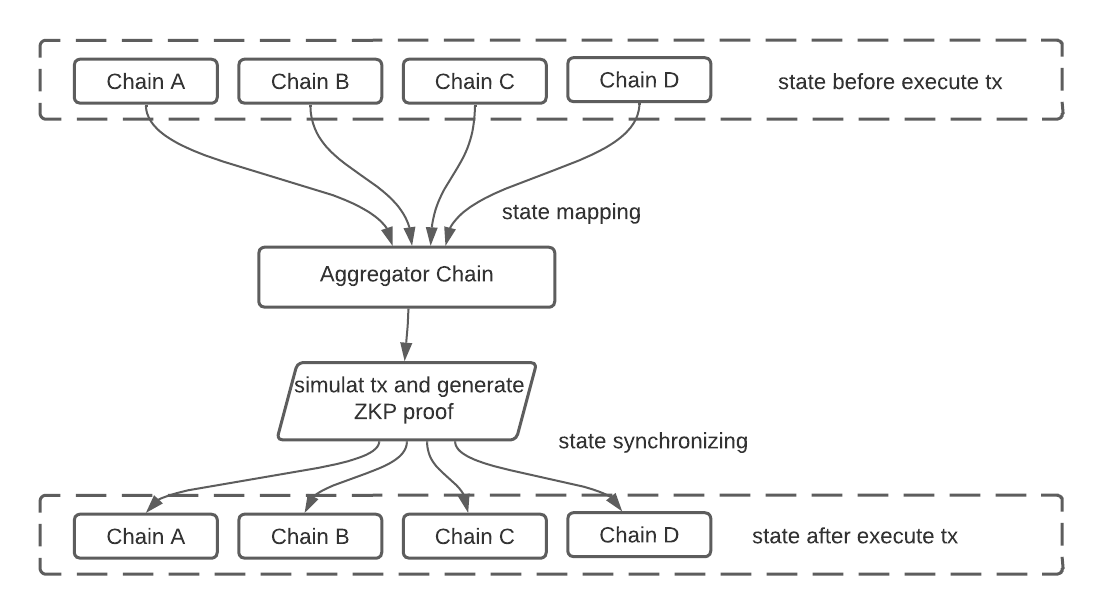
\includegraphics[scale=0.4]{main-idea}}
\caption{Overview of \dprotocol}\label{main-idea}
\end{figure}
\begin{enumerate}[leftmargin=*]
\item We map the local state $s_i$ of each block chain $C_i$ into our newly introduced aggregator chain to form a global state $s = \langle s_0, s_1, \cdots \rangle$.
\item We perform a simulating run of the bundled transactions over $s$ on the aggregator chain to get a resultant state $s' = \langle s_0, s_1, \cdots \rangle$ and create zero-knowledge proofs to convince each native chain $C_i$ that after the bundled transaction has been executed, their local state has to be changed to $s_i'$.
\item We ask every native chain $C_i$ to change their local state by providing them the resultant state $s_i'$ and the zero-knowledge proof.
\end{enumerate}

\smallskip Below we present a brief picture of our solution by a case study (see Section \ref{chp:case-study}) of the standard transfer and explain how zero knowledge is applied so that the safety, liveness, and permissionless properties hold. In Section \ref{chp:protocol-details} we describe each component in detail and then we explain the trust base of our solution and prove that under the trust base our solution has a full guarantee of safety, permissionless and liveness properties (see Section \ref{chp:properities}).

%Regarding the permissionless, we need to ensure that neither safety and liveness properties can be affected when introducing new decentralized nodes in \dprotocol. Since the safety is enforced by ZKP(zero knowledge proof), it is sufficient to prevent new joined nodes from ordering transactions unfair. Therefore we use BFT(Byzantine Fault Tolerant) consensus algorithm and permissionless property relies on that two-thirds of the nodes of the aggregator chain are honest.


\section{Protocol Overview}
\label{chp:case-study}
As a case study, we focus on a standard simplified asset transfer process from Alice on chain $C_A$ to Bob on chain $C_B$ through a liquid provider in $C_A$ and $C_B$ \cite{introdefi}. 

%\begin{figure*}[!ht]
%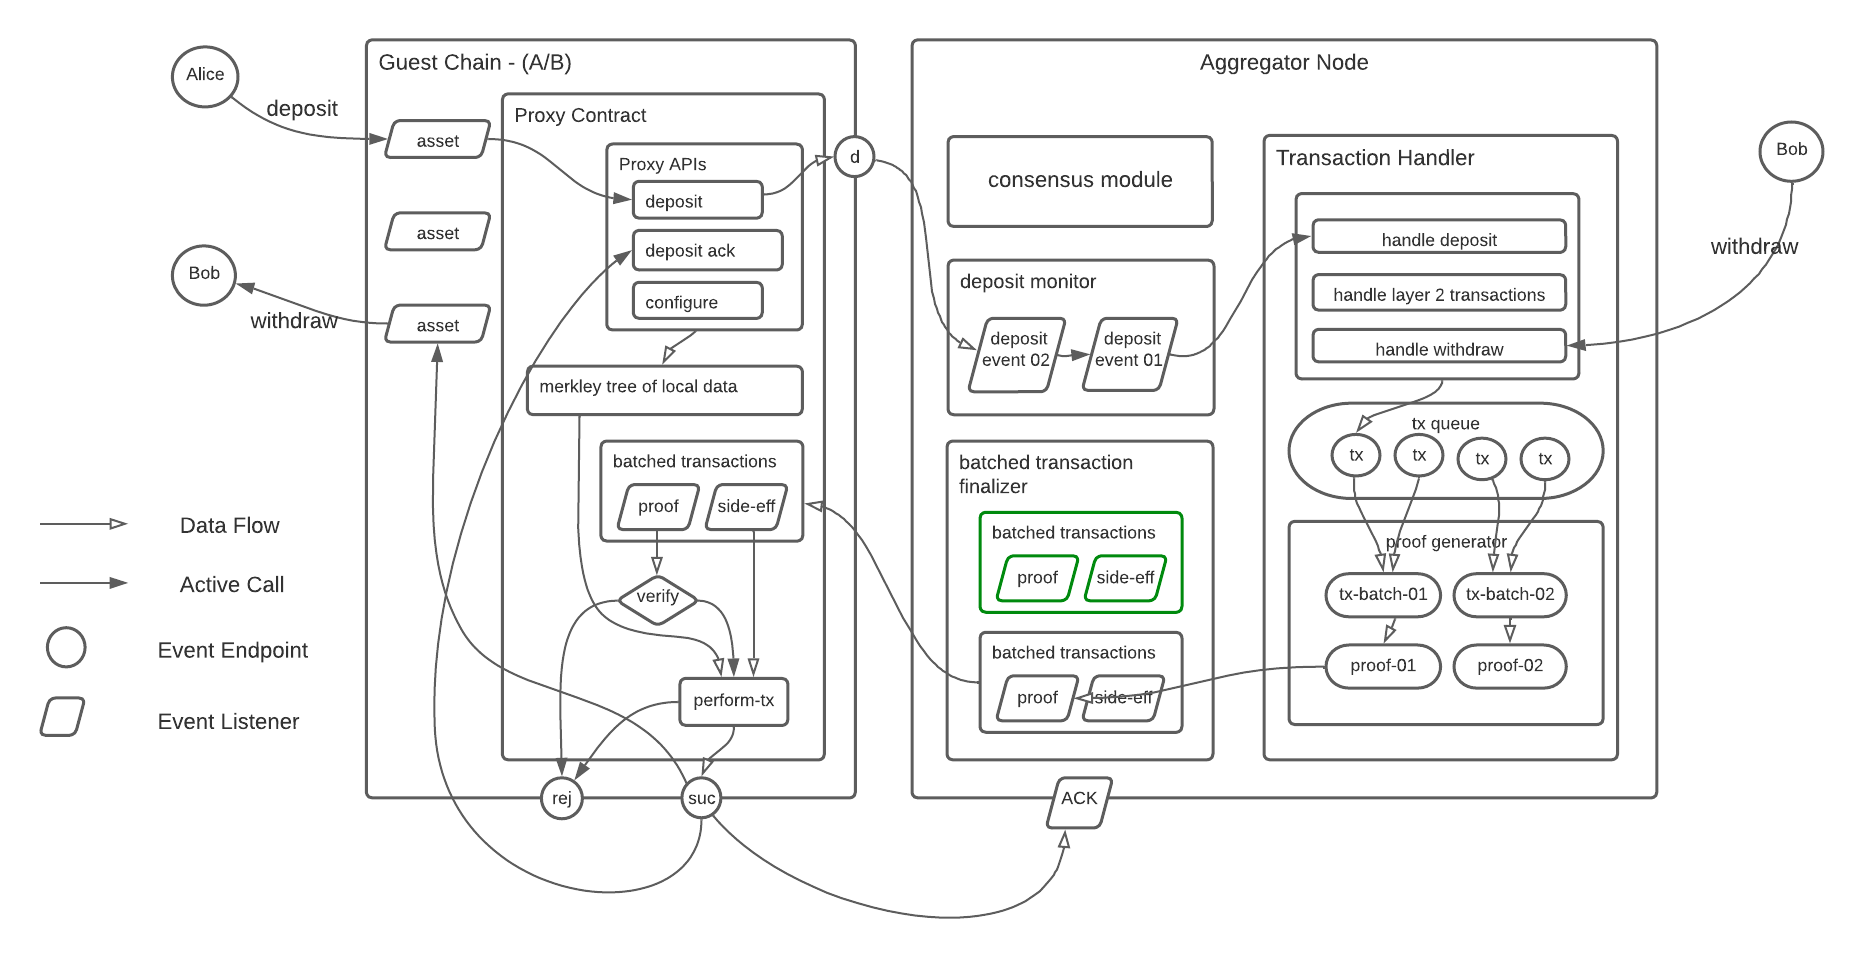
\includegraphics[scale=0.6]{case-study}
%\caption{Case study of a cross-chain token transfer}
%\label{case-study}

%\end{figure*}

\subsection{State Abstraction}
First, 
%we define the native-chain set in the bundled transfer transaction to be $\mathbb{C} = \left\{C_A, C_B\right\}$. As Alice has some assets on $C_A$ and Bob has some assets on $C_B$ and a liquid provide has assets both on $C_A$ and $C_B$, 
we abstract our local state $s_A$ of $C_A$ and $s_B$ of $C_B$ separately as follows.

\begin{lstlisting}[escapeinside={(*}{*)}, basicstyle=\small, xleftmargin=0.6cm, backgroundcolor = \color{lightgray}, numbers=left]
(*$s_A$*) = state {
    alice: number
    lp: number
}
(*$s_B$*) = state {
    bob: number
    lp: number
}
\end{lstlisting}

Now, as we have described in Section \ref{prelimiary}, the underlying global state $s$ of transfer is a tuple of $C_A$ and $C_B$:
\begin{lstlisting}[escapeinside={(*}{*)}, basicstyle=\small, xleftmargin=0.6cm, backgroundcolor = \color{lightgray}, numbers=left]
s = state {
    sa: (*$s_A$*),
    sb: (*$s_B$*)
}
\end{lstlisting}

Second, the bundled transfer transaction $tx$ is defined as a function on global state $s$ as follows:

\begin{figure}[!ht]
\begin{lstlisting}[escapeinside={(*}{*)}, xleftmargin=0.6cm, basicstyle=\small, backgroundcolor = \color{lightgray}, numbers=left]
function transfer(amount) {
  transfer(Alice, amount, lp);
  
  s.sa.alice = s.sa.alice - amount;
  s.sa.lp = s.sa.lp + amount;
  
  s.sb.bob = s.sb.bob + amount;
  s.sb.lp -= amount;
  
  if(s.sb.lp > amount) {
    transfer(lp, amount, Bob);
  }
}
\end{lstlisting}
\caption{Transfer Transaction}
\label{fg:transfer}
\end{figure}

where line 2 can be treated as the invoke transaction on $C_A$, line 4-12 are bundled transactions that will be simulated on the aggregator layer and line 11 is the side effect on $C_B$.

Unlike other bridge-like solutions which performs 2-5 on $C_A$, 7-11 on $C_B$, and using relayers to synchronize two parts, \dprotocol simulates the transaction in the aggregator chain on global state $s$ and then uses ZKP of the simulation to convince native block chains to update their local states.

In our protocol, we divide the life cycle of the transfer transaction into four stages: consensus stage, operating state, proving stage and finalizing stage
%(see Figure \ref{case-study}).



\smallskip\noindent\emph{Consensus Stage.}
A user Alice transfers a certain amount of money into a proxy contract (line 2 in Figure \ref{fg:transfer}). After the contract handles the invoke transaction, it commits the amount into its table of unfinalized invoke transactions and emits an event. This emitted event will get monitored by \dprotocol Node and triggers the consensus stage.

In the consensus stage, a node who wins the voting protocol generates two ZK proofs. One proves that the event is real and the other proves that the winner is picked by the consensus algorithm. (This can prevent a node systematically ignore transactions it ignores). Also, Alice is allowed to withdraw the unfinalized amount after a certain amount of time (based on blockheight) (see Section \ref{chp:protocol-details} for more information about encoding consensus into ZKP circuits).

\smallskip\noindent\emph{Simulating stage:}
Once a transaction is ready to execute, it will be simulated by the voted aggregator chain node so that a new resultant global state $s'$ can be calculated from the initial state $s$. Recall that $s$ is got by aggregating states $s_i$ from different native blockchains $C_i$. It follows that by projecting $s’$ back onto different partial states, we know how to update the local state $s_A$ and $s_B$ on $C_A$ and $C_B$ accordingly.

\smallskip\noindent\emph{Proving stage:}
After the \dprotocol node finishes simulating the execution of our particular transfer transaction, it will create a zero-knowledge proof to show how to update all the partial states on $C_A$  and $C_B$.

Compared to traditional side-chain solutions, which require audit nodes to validate transactions and may suffer from majority attacks, \dprotocol uses ZKP to enforce that the simulation is carried out on predefined functions (in this case, line 4-12 in Figure \ref{fg:transfer}). Thus even the majority of the audit nodes are hacked, they can only perform attacks that lead to deny-of-service of some of the transactions. Later in Section 4 we will prove that the DOS attack is theoretically infeasible once we have a permissionless aggregator chain and any node of it can helping executing and finalizing bundled transactions if it can provide ZKP for the simulation.

Once the $tx$ was fully performed, the aggregator chain will broadcast this transaction together with its proof to native-chain $C_A$ and $C_B$.

\smallskip\noindent\emph{Finalizing Stage}:
After a zero-knowledge proof, a simulation of our transfer is generated, and the voted aggregator node will call a special finalizing contract on the native blockchains $C_A$ and $C_B$ which will verify the proof and then perform the side-effects of each sub transaction accordingly.

In the case of a transfer, after the proof is verified, $C_A$ and $C_B$ will change their local state accordingly and on $C_B$, a side effect (line 11) is performed so that Bob receives the transferred assert correctly (This amount must equal to the amount transferred by Alice otherwise the zero-knowledge proof will not be valid).


%\subsection{Application of the Zero-Knowledge Proof Technique}
%For the correctness of the simulation, the verification of ZKP on verify contract makes sure that all transactions are performed under predefined functions and the resultant state is correctly calculated (Merkle root hash is pinned). Since the transfer on $C_B$ is performed at the end, it makes sure that the amount being about to withdraw is a consequence of valid transaction simulation.

%For the correctness of the deposit monitor, ZKP is used to make sure the monitored event is pined to the native-chain root hash \cite{sidechainzkp} so that the custody of transferred tokens is reported to the aggregator node honestly. 

%For the liveness and permissionless property, \dprotocol utilizes a group of nodes and they use a BFT consensus algorithm to vote the next block generator. The ZKP of the voting result is then used to convince the native blockchains that the consensus algorithm on the aggregator layer is enforced (see \ref{consensus-stage}).

%\subsection{Cost of Zero-Knowledge Proof Verification}
%Regarding the cost problem of state pinning, since \dprotocol uses batched transactions to reduce the cost of the signature check and SNARK proof check, the problems of the high cost of state pinning and signature check can be reduced to an acceptable level.
\section{Protocol Details}
\label{chp:protocol-details}
The target of \dprotocol is to provide a universal layer to simulate and synchronize the global state between various blockchains which support smart contracts. This universal layer is organized as a blockchain of \dprotocol nodes and each node contains four abstract components: storage component, transaction handler and simulator, native chain monitor and transaction finalizer.  Besides aggregator nodes, we also need to 
integrate native proxy contracts on native blockchains so that they can invoke transactions and update the local state accordingly.


\subsection{\dprotocol Node}
In a blockchain setting, we combine the finalizer, storage component, transaction handler and native chain monitor (everything except proxy contracts on native blockchains) together and equip it with an extra consensus component into a \dprotocol node. These distributed \dprotocol nodes form a blockchain that works together to synchronize and alter states between native blockchains. Each component in the node performs the following task:

\begin{enumerate}[leftmargin=*]
\item Chain Storage Component:
    \begin{itemize}
    \item store the global state.
    \item store the Merkle root hash of the whole state.
    \item store the valid voter list and the Merkle root hash of all voters.
    \end{itemize}
\item Transaction Handler and Simulator.
    \begin{itemize}
    \item order aggregator chain transactions under consensus.
    \item process transactions and update the whole state.
    \item emit transaction events (with execution order).
    \end{itemize}
\item Native Chain monitors:
    \begin{itemize}
    \item handle event emitted by invoke transaction of a bundled transaction.
    \item handle event emitted by revoke.
    \end{itemize}
\item Transaction Finalizer:
    \begin{itemize}
    \item calculate transaction execution proofs.
    \item calculate proofs of consensus.
    \item submit proofs to a guest chain for validation and finalization.
    \end{itemize}
\item Consensus component:
    \begin{itemize}
    \item perform consensus algorithm (voting block generator).
    \item calculate ZKP of the consensus algorithm.
    \item generate and prepare block.
    \end{itemize}
\end{enumerate}

Finally, proxy contract on the native-chain is also an important component of \dprotocol as it is used to maintain the partial state of a particular native chain by performing proof verification, state updating and processing the side effects of each transaction during the finalizing stage.  

As an example, suppose that we have two blockchains $C_{A}$ and $C_{B}$. Then our single \dprotocol involves the following entities (see Figure \ref{protocol-components})
\begin{figure}[!ht]
\centerline{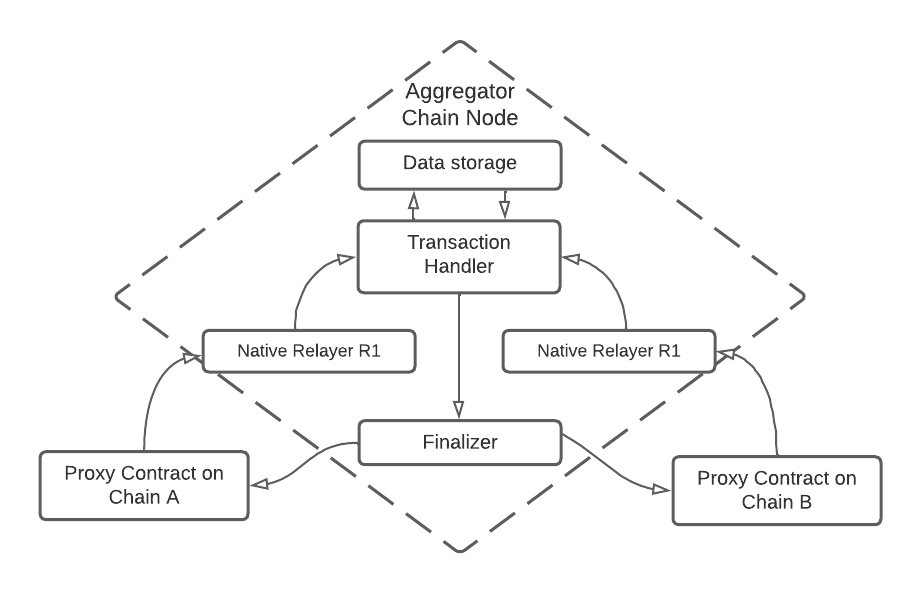
\includegraphics[scale=0.5]{components}}
\caption{Protocol components}
\label{protocol-components}
\end{figure}

%\noindent with each component performs the following functionalities:
%\begin{itemize}
%\item  Proxy smart contracts $\mathcal{A}$ and $\mathcal{B}$ on $C_A$ and $C_B$ (Trusted).
%\item  A transaction handler that handles and simulates transactions.
%\item  A storage component that tracks the global state.
%\item  Monitors $\mathcal{R}_A$ and $\mathcal{R}_B$ to monitor invoke (or revoke) transaction events for $C_A$ and $C_B$ and reports them to the transaction handler.
%\item  A finalizer that communicates with proxy contracts to finalize transactions.
%\end{itemize}
%\smallskip
%Moreover, 

\subsection{Transaction Lifecycle}
In \dprotocol the global state is compressed as a Merkle hash tree and pinned in all the guest chain proxy contracts. A bundled transaction $tx$ is a set of operations $tx_i^k: s_k \mapsto s_k'$. By defining how the local state $s_k$ of the application can be changed through $tx_i^k$, $tx$ can be treated as a function on the global state $s$. For a transaction to be successfully executed in \dprotocol, it undergoes the following four stages: (see Figure \ref{transaction-fifecycle}).
\begin{figure}[!ht]
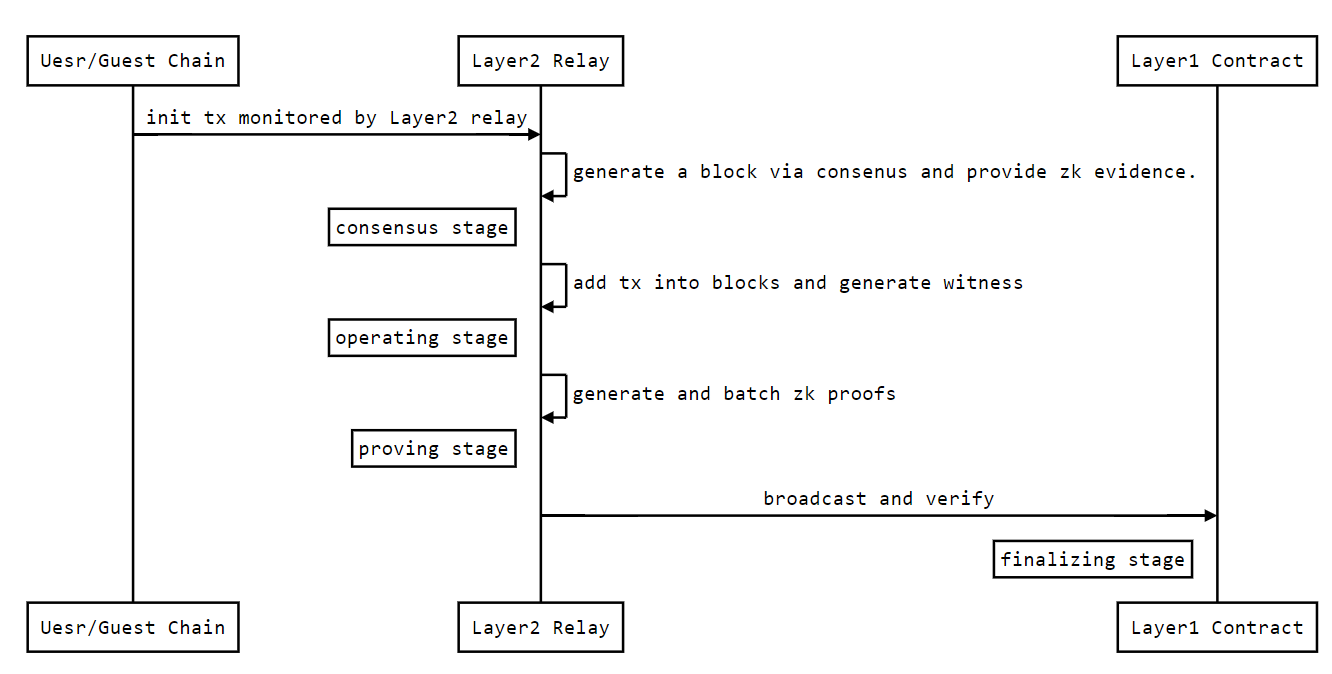
\includegraphics[scale=0.44]{consensus-sequence.png}
\caption{Transaction Life Cycle}
\label{transaction-fifecycle}
\end{figure}
\begin{enumerate}[leftmargin=*]
\item \emph{Consensus Stage:} As a decentralized protocol, a transaction will not get handled until it is collected in a block. Each block is produced by an elected node under a pre-defined consensus algorithm. A node that wins the consensus game needs to provide a ZK proof which will later be used as evidence to finalize all transactions within the block on the guest proxy contract.

\item \emph{Operating Stage:} At the operating stage, an operation is simulated on \dprotocol and changes the global state thus changing the Merkle root. During the simulation, all the information needed to create a ZKP for the simulation is prepared and stored. Since all transactions are handled sequentially regarding their order in a particular block, their proofs are stored in the same order so that they can be batched in the proving stage. 

\item \emph{Proving Stage:} After the operating stage, the finalizer will generate all the proofs for every transaction and compress proofs into a single ZKP proof. This proof is then appended after the transaction information in the block with an updated Merkle tree hash. 
\item \emph{Finalizing Stage:} Once the proof of batched operation sequence is generated by the finalizer, it will broadcast to various underlying blockchains. The blockchain needs to verify the proof, perform side-effects, and then emit acknowledge event to finalize the transaction.
\end{enumerate}

\subsection{Protocols in Each Stage}
\textbf{Consensus Stage.}
\label{consensus-stage}
A consensus algorithm is a common process in blockchain to achieve agreement on value or state among distributed nodes. A consensus algorithm is critical in systems that contain permissionless unreliable nodes. In \dprotocol we need a consensus algorithm to decide the following:

\begin{enumerate}[leftmargin=*]
\item Decide the order of the bundled cross-chain transactions.
\item Enroll and identify a valid node.
\item Vote a node to produce the next block and finalize the transactions in it. 
\end{enumerate}

In \dprotocol we use a modified PBFT \cite{castro1999practical} consensus algorithm between chain nodes to vote for a block generator. Recall that PBFT consensus consists of three phases: Pre-preparation, Preparation and Commit. At the Pre-preparation stage, the primary node is responsible for verifying the requests and generating corresponding pre-preparation messages. Then, in the preparation stage, the primary node will broadcast pre-preparation messages to all Replica nodes. After receiving the messages, Replica nodes will verify those pre-preparation messages and then broadcast a corresponding prepared message.

The final step in \dprotocol is carried out on native chains thus the results are not broadcast back to Replica nodes but broadcast to native chain nodes and verified there. Moreover, in addition to verifying that the results are correctly calculated, we also need to convince the guest chain that our generated blocks are produced under the consensus protocol as well. Usually, since the native chain does not attend the consensus algorithm in the aggregator-chain, it has the problem of checking whether the transaction results are reported from a fairly picked node. Thus we need to encode the consensus algorithm and its result into a zero-knowledge proof so that we can confirm the guest proxy contract that the block contains all transactions is generated legally. The consensus result together with its ZKP proof is stored in a newly generated block.

%as described as follows (see Figure \ref{block-layout}). 

%\begin{figure}[!ht]
%\begin{center}
%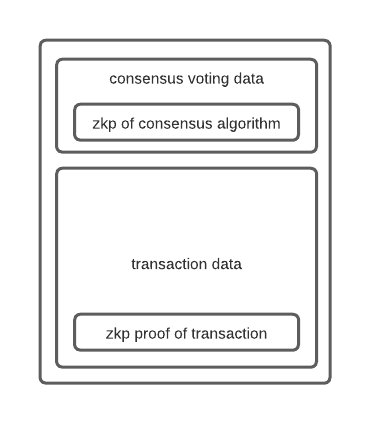
\includegraphics[scale=0.5]{block-data-layout}
%\end{center}
%\caption{Data layout of an aggregator block}
%\label{block-layout}
%\end{figure}

To satisfy all the above requirements, our modified PBFT approach still consists of three phases but each phase is slightly modified as described below.

First, at the pre-preparation stage, a node needs to be registered as a valid block generating candidate and broadcast the ZKP of the validation to other nodes. During the process of voting (preparation stage), each aggregator chain node in the consensus stage places a vote and sends a signature of the vote to their voting target. Suppose that two-thirds of the nodes in the system are honest then it follows that only one potential node will win the voting game and this particular node is authorized to produce a block.

Second, after a certain node gathers enough voting messages, instead of broadcasting the result, the winner node will calculate the ZKP of our consensus algorithm and put it into its generated block. This ZKP will later be used to convince the native blockchains that a batched transaction proof is sent from a legally voted node. Once the proof is attached to the newly generated block the winner node will start producing transactions (see Figure \ref{vote-sequence}).

\begin{figure}[!ht]
\begin{center}
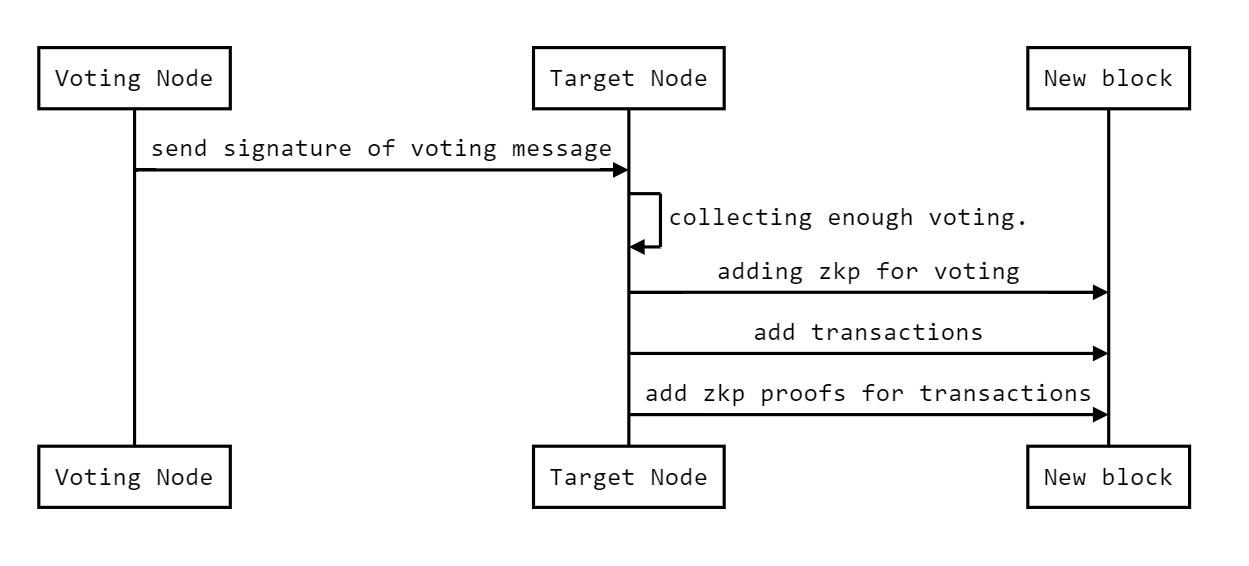
\includegraphics[scale=0.4]{vote-sequence.png}
\caption{Voting process during consensus}
\label{vote-sequence}
\end{center}
\end{figure}

In the end, the winner node will broadcast the generated block to the native blockchains. \dprotocol proxy contract on the native blockchain will verify and finalize this block and update its local state accordingly.

\dprotocol targets to build a permissionless chain that everyone can join the aggregator chain to helping to synchronize bundled cross-chain transactions. This means we need to provide a protocol to register and remove a valid voter. To achieve that, \dprotocol keeps a Merkle tree of all valid nodes by tracking their public keys as Merkle tree data nodes and anyone can register to be a valid node by registering itself as a new Merkle tree leaf. Also, for an aggregator node to vote for the next block producer, it has to prove the target it votes is a valid Merkle tree node (a registered valid node) first and then sign and send his voting ticket to the voted node. More precisely anyone can do the following:
\begin{enumerate}[leftmargin=*]
\item Register a node for voting:
    Node registration is an aggregator chain transaction that updates the Merkle tree of all valid voters on the aggregator chain and has the side effect of updating the Merkle tree root hash of nodes in the guest proxy contract. It is the responsibility of every aggregator node to keep the registration tree updated so that the root hash is consistent with the pinned hash in the proxy contract. 

\item Validate a voter:
    When a node receives voting from another node, it needs to validate that the sender is a valid voter. If the sender is an invalid node (eg, a malformed node without registration) then proof of sufficient voter will fail at the stage of finalizing thus wasting the computing source of the node who voted.

    Recall that all the valid voters are arranged in a Merkle tree whose root hash is pinned in the guest proxy contract. The voter needs to provide identity proof (in the form of ZK proof) to show that his public key (or voting address) is one of the Merkle tree leaf nodes.
    
    Once a node receives voting from voter $V$, it needs to verify the identity proof of $V$ first before it pushes it to the list of its supporters for the next block generation round.

\item Send a valid vote ticket:
    A voting ticket contains two parts, a signature, and validation proof. The signature is signed from the current block height together with the Merkle root hash of all valid voters. The validation proof is a zero-knowledge proof that proves that the voter is one of the valid voters. 
\end{enumerate}

\smallskip\noindent\textbf{Simulation Stage.}
After a node is voted as a block generator, it can start collecting transactions from various sources. In ZK Multi-Blockchain Aggregator, transactions are submitted to aggregator node, via three sources (see Figure \ref{simulation-stage}).

\begin{figure}[!ht]
\begin{center}
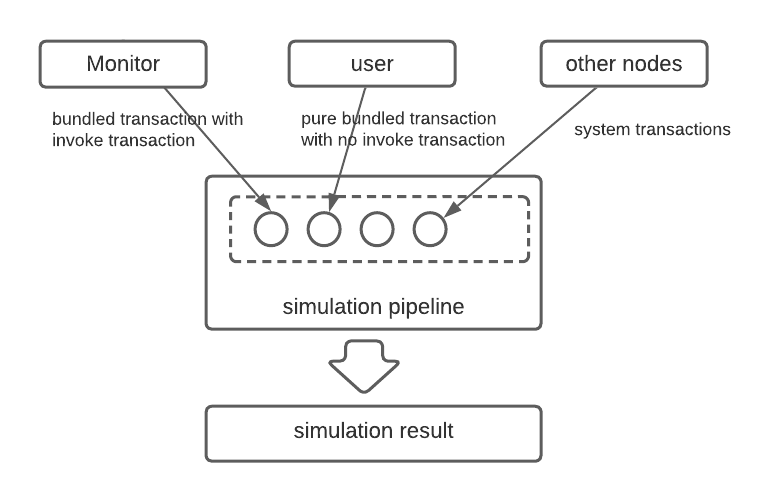
\includegraphics[scale=0.6]{simulation-pipeline.png}
\end{center}
\caption{Simulation stage}
\label{simulation-stage}
\end{figure}

\noindent\textit{1. The pure bundled transaction that does not contain an invoking transaction:} A pure bundled transaction is supposed to be sent directly to \dprotocol nodes and all its internal sub-transaction should either all succeed or fail. Notice that whether each sub-transaction will succeed (or all fail) can be determined via simulation in the aggregator node, the finalizer only finalizes succeeded transactions.

\noindent\textit{2. The bundled transaction that start with an invoking transaction}: This kind of bundled transaction is similar to the pure bundled transaction except that its first sub-transaction (and only the first sub-transaction) can not be simulated by the aggregator node. When handling this kind of transaction, the first transaction is executed on the native-block chain first and the monitor of the aggregator node monitors the result of the first transaction. If the first transaction is succeeded, the monitor submits the following transaction to the aggregator node. If not, the monitor submits a revoke transaction to the aggregator which will trigger a revoke of the invoking transaction just performed on the native-chain.

\noindent\textit{3. System transactions}: These kinds of transactions are submitted by aggregator nodes and it contains voting transaction, voter registration transaction, voter quit transaction, etc.

\smallskip\noindent\textbf{Proving Stage.}
As we discussed before, we simulate bundled transactions of the global state on the aggregator chain node and each bundled transaction is equivalent to a function $f: s \mapsto s'$. Since the global state is pinned on the native-chain by the Merkle hash root $h(s)$ of the state, a zero-knowledge proof of bundled transactions $tx$ is a proof that ensures the Merkle hash root of the result state $s' = f(s)$ is valid. 

\begin{figure}[!ht]
\begin{center}
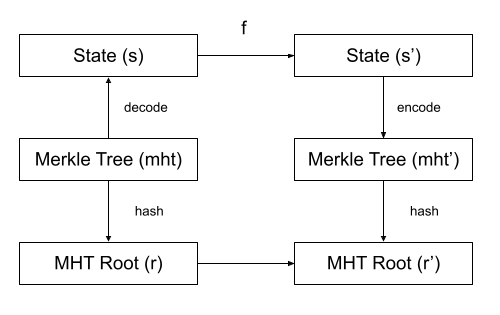
\includegraphics[scale=0.8]{circuit-state-refine}
\end{center}
\caption{State refine of transaction circuit}
\label{circuit-refine}
\end{figure}

For example (see Figure \ref{circuit-refine}), suppose that, before the transaction, state $s$ is encoded into the Merkle hash tree $mht$ which has root hash $r$ and after simulating the transaction the state changes to $s' = f(s)$. Also, suppose that this new state was stored in the aggregator chain storage in a format of updated Merkle tree $mht'$ whose new root hash is $r'$.
Then it follows that we need to create a zero-knowledge proof to show that the following constraints hold.
\[ constraints = \begin{cases}
    r = root(mht(s)) \\
    r' = root(mht(s'))\\
    mht(s') = mht(f(s))
\end{cases} \]
where the first two constraints are constraints about the state before and after the transaction and the last constraint is about the simulation of the function $f$.

%Moreover, $f$ can be treated as a sequence of leaf updates of the Merkle tree of state $s$. For each leaf update, suppose that $P_k = [p_0, p_1, p_2 \cdots p_n]$ is the MTI of an updated leaf of data $D_k$. It follows that to calculate the root hash after the modification of data of $D_k$, we need to calculate a new hash root at each level from $p_n$ to $p_0$ by the formula
%$$
%    H_k(p_k) = hash(H(p_{k+1}^0), H(p_{k+1}^1),\cdots) 
%$$
%where $a_i = p_{k+1}^{j}$ are nodes who have the same parent $p_k$ as $p_{k+1}$ \cite{liskov2005updatable}. A full transaction $tx$ is a data %transform function $f$ performed on multiple Merle leaf nodes. 

In \dprotocol node $f$ is defined as a combination of the following:

\begin{enumerate}[leftmargin=*]
\item Simple Merkle tree leaf update.
\item Predefined functions that have predefined ZKP circuits.
\item Cryptographic functions including signature functions and hash functions.
\end{enumerate}

\smallskip\noindent\textbf{Finalizing Stage.}
We know that a bundled transaction $tx$ is a state transformer over global state $s$ and is composed of a sequence of sub-transactions $tx^j_{k_j}$ on $C_{k_j}$. During the finalizing stage, \dprotocol mainly performs three things. First, it checks the ZKP of the consensus algorithm to make sure the block was generated by a valid block producer. Second, it checks the ZKP of the simulation of $tx$ so that the proxy contract can safely update the local state on $C_{k_j}$. Third, the proxy contract performs the side effects of $tx^j_{k_j}$ on $C_{k_j}$ (e.g., if a user would like to withdraw some asset from the aggregator chain to the guest chain, then during the finalizing procedure a transfer from the guest chain proxy contract to the target account of the withdrawal is executed).

\subsection{Guest Proxy Contract}
Guest Proxy Contract contains two parts: \emph{guest chain interface} and \emph{verification} interface (see Figure \ref{local-state}). Both of them manipulate the local state of guest chain. The guest chain interface includes invoke and revoke which allows guest chain users to invoke or revoke a message. The verification interface is called by \dprotocol node to finalize transactions.

\begin{figure}[!ht]
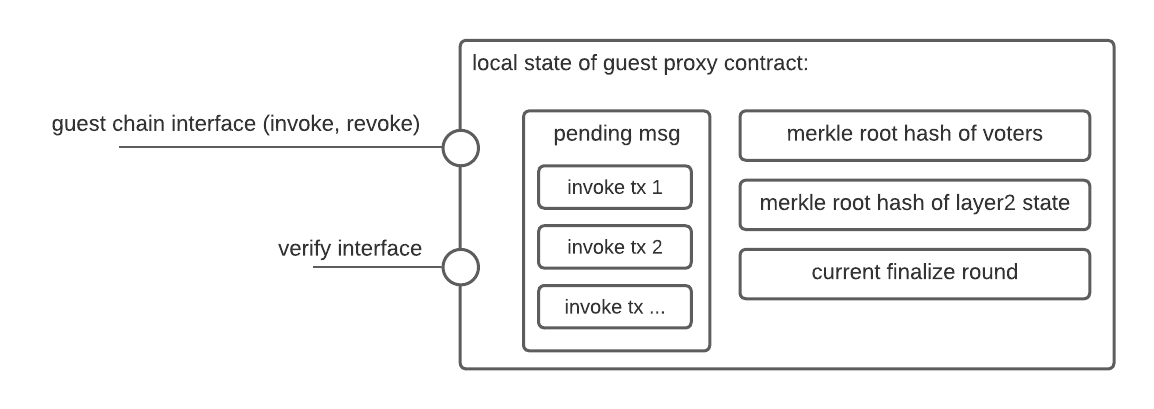
\includegraphics[scale=0.15]{proxy-local-state.png}
\caption{Local state of guest proxy contract}
\label{local-state}
\end{figure}

\subsubsection*{Guest chain interface.}
When a user invokes a {\bf guest chain interface}, the transaction info with the current block height ($h$) is recorded in the pending queue of the guest local state. The user who performed invoke transaction can revoke his invocation any time when the transaction remains in the pending queue after a fixed amount ($\delta_h$) of the block. This means \dprotocol nodes have to notice and handle this event and finalize this event within $\delta_h$ blocks.

%\begin{figure}[!ht]
%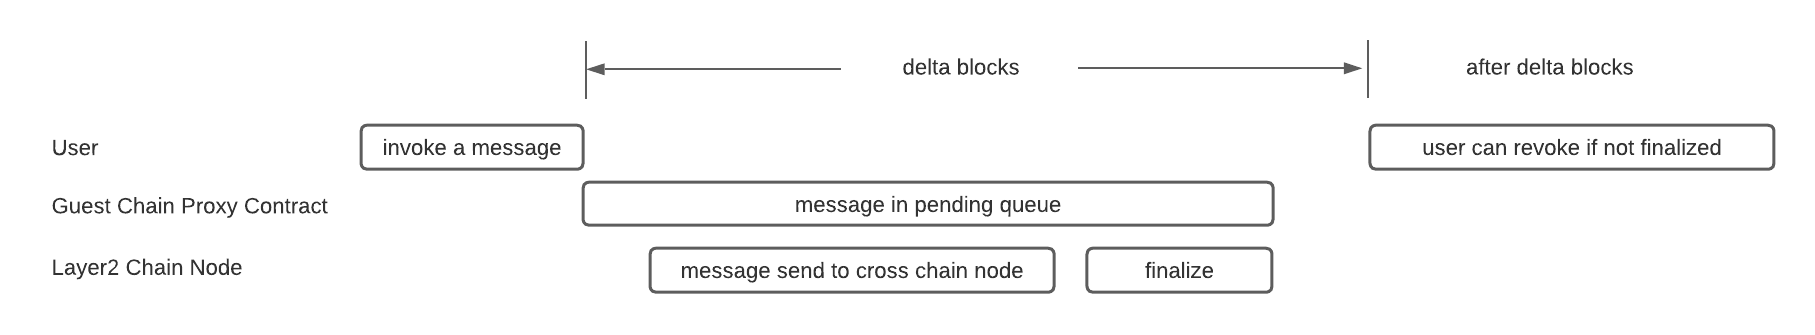
\includegraphics[scale=0.125]{whole-process}
%\caption{Time window for finalizing a block}
%\label{time-window-finalizing}
%\end{figure}

\subsubsection*{Verification Interface.}
The verification interface verifies the ZK-SNARK proof generated by the aggregator chain node (see Section 2.5).
\begin{figure}[!ht]
\begin{code}
function verify(
  uint256 l2account,
  uint256[] memory tx_data,
  uint256[] memory verify_data, // ZK proofs 
  uint256 vid,
  uint256 nonce,
  uint256 rid
)
\end{code}
\caption{Verification API in Native Blockchain}
\label{fig:verify-api}
\end{figure}

Recall that only the winner of the voting consensus of the current finalizing round ($rid$) is authorized to invoke the verification interface at round $rid$. It follows that the verification function (see Figure \ref{fig:verify-api}) first checks the voting proof to ensure that the sender is the winner of round $rid$ and then checks every transaction encoded in {\it tx\_data} is executed honestly via verifying the ZK proof encoded in {\it verify\_data}. If both check pass, the guest contract will perform all the side-effects of transactions on the guest chain accordingly (see Figure \ref{sideffects}).

\smallskip\noindent\emph{Types of transaction side-effects during finalization:}
\begin{itemize}[leftmargin=*]
\item \emph{Invoke:}
    An invocation $tx$ on the aggregator chain must be related to an invocation call on a guest contract, since every time a guest chain invocation will cause a record of pending invocation to be added to the pending list in the local state of the guest contract.
    Once a invoke $tx$ is verified, the side effect of that $tx$ is removing the invocation record in the pending invocation list.
    Once an invocation was removed from the pending invocation list, its sender loses the capability to withdraw it.

\item \emph{Callback:}
    The callback is a special transaction that is invoked through \dprotocol Node which tries to trigger a certain callback function from \dprotocol Chain to guest Chain.
    Once a callback $tx$ was verified, its side effect is to call a related guest contract API according to the $tx$ information.
    Withdraw is a special case of callback that calls the transfer API.

\item \emph{Generic Transaction:}
    All bundled transactions are simulated in aggregator nodes and the global state is pinned to the guest contract. So there is no other side-effect during the process of finalization for generic transactions.
\end{itemize}
\subsection{Guest Chain Monitor}
Guest chain monitor is responsible for monitoring guest chain events and notifying aggregator chain $tx$ handlers by forwarding them. The guest chain monitor needs to sign the event with its consensus ID. If a voted \dprotocol node failed to finalize its transactions in the guest chain proxy contract, then it either fails to calculate a correct ZKP proof of transactions and voting result or it does not pass the checks in the side-effect of invoking transactions in the guest contract. In the later case, the failed node could be a malicious node that provides invoking transactions that do not exist on the guest chain.  
\begin{figure}[!ht]
\begin{center}
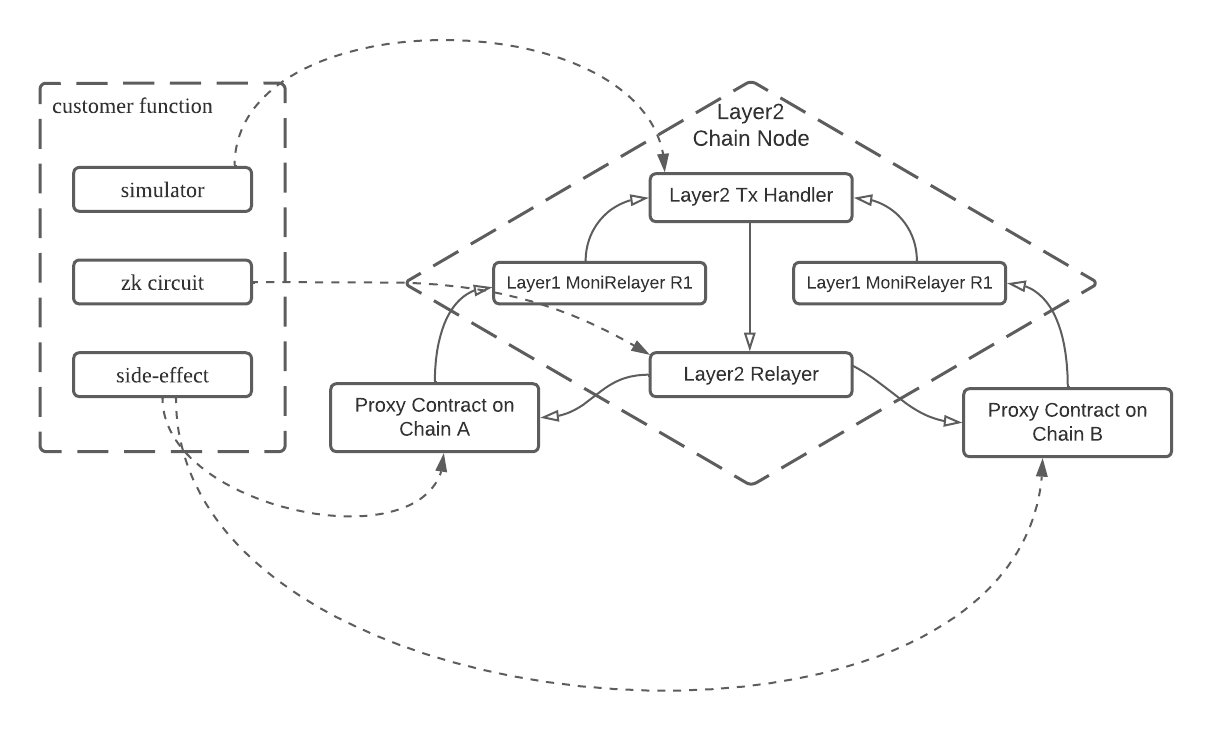
\includegraphics[scale=0.4]{side-effects}
\caption{Perform side effects of a bundled transaction}
\label{sideffects}
\end{center}
\end{figure}

\section {Properties the Protocol Garantees}
\label{chp:properities}

%Delphinus cross-chain is a decentralized platform that anyone can join network to help synchronize cross-chain bundled transactions. Thus to show that Delphinus cross-chain is a permissionless system, we need to show that although any running Delphinus cross chain node can play the role of synchronizing cross-chain transactions, the data stored in Delphinus cross chain is consistent and all local data stored in distributed nodes converges.


\subsection{Permissionless Property}
\dprotocol is a decentralized layer that anyone can join network to help synchronize cross-chain bundled transactions. To enforce permissionless, we need to show that although any running node can play the role of performing multi-blockchain transactions, the data stored in the chain is consistent and all local data in distributed nodes converges.

Given a group of bundled transactions $\mathbb{T} = \left\{tx_i\right\}$ submitted simultaneously, a valid trace from a start point of global state $s$ is a sequence of global state $s_0, s_1, \cdots s_n = s'$ such that $s_{k+1} = tx_k(s_k)$ where $tx_k \in \mathbb{T}$.

It is obvious that different order of $tx_k$ from the same $\mathbb{T}$ can lead to different valid traces. Thus we need a consensus algorithm so that all attending nodes in the \dprotocol can vote for a unique block producer to generate a globally valid trace.

We uses a Merkle tree to record all the valid voting nodes and pin the root hash of the Merkle tree in native blockchains. For a new node to register itself as a valid node, it needs to fire a register transaction on the aggregator chain and synchronize the root hash themselves before vote.

To vote a node, a voter needs to sign a voting message and send the signed voting message to the target it votes. Inside the message, it contains the Merkle root hash of all valid voters and target's public address. Once a node receives sufficient amount of voting tickets it will produce a zero-knowledge proof which shows that the total number of tickets reaches two-thirds of the total number of voters and all of them has the correct Merkle root hash. 

As mentioned in Section \ref{chp:protocol-details}, after the winner node calculated the ZKP proof of all received signatures, it can start producing a block that represents a valid sequence of bundled transactions $\mathbb{T}$. This process is executed locally and the block producer can pick any order of $tx_i$ in the final sequence as long as it can generate a ZKP proof of the simulation.

\begin{figure}[!ht]
\begin{center}
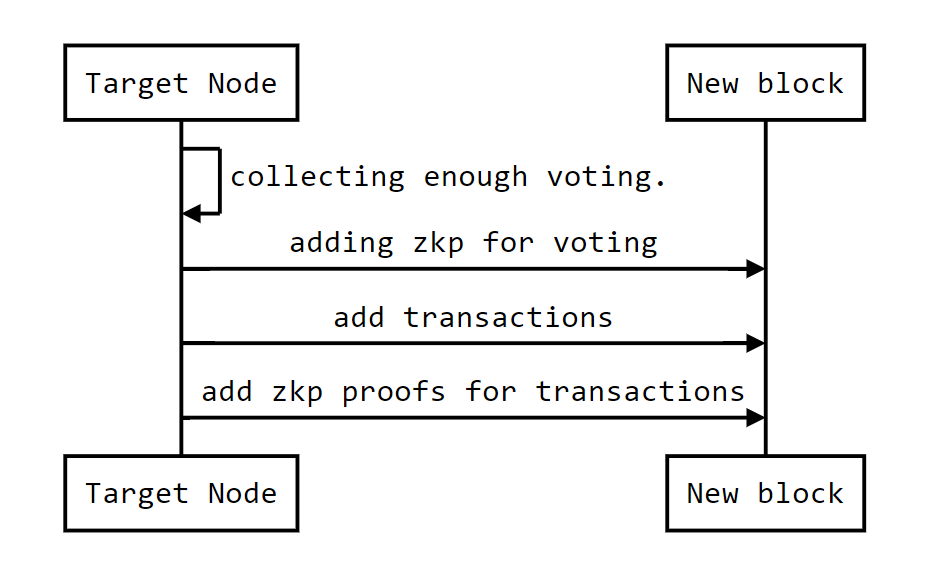
\includegraphics[scale=0.4]{produce-block.png}
\end{center}
\caption{Produce a block after voting}
\label{produce-block}
\end{figure}

Once the block was generated, it needs to be sent to the native block chain $C_i$ to finalize before it can be recorded in the Delphinus aggregator chain ledger. 

As the consensus algorithm solves the ordering problem, it remains to make sure the winner node can not produce a partially finalized block (finalize the block to a subset of the native blockchains). Thus we need a strategy to continue finalizing the block even if the winner node quit after generating the block. To achieve this, we simply record the proof data on the native chain $C_i$ during finalization so that if a block was synchronized partially, then all Delphinus nodes will notice the recorded proof and can continue broadcasting the proof until it is fully synchronized. Moreover, if the winner does not finalize its block to any of the native chains, then we relies on the liveness property to make sure another block generator can be voted (see Section \ref{chp:sub:liveness}).

\subsection{Liveness Property}
\label{chp:sub:liveness}
We abstract the state transition diagram as follows (see Figure \ref{state-transition}), and we would like to show that all intemediate states leads to either full finalize state or skip state.
\begin{figure}[!ht]
\begin{center}
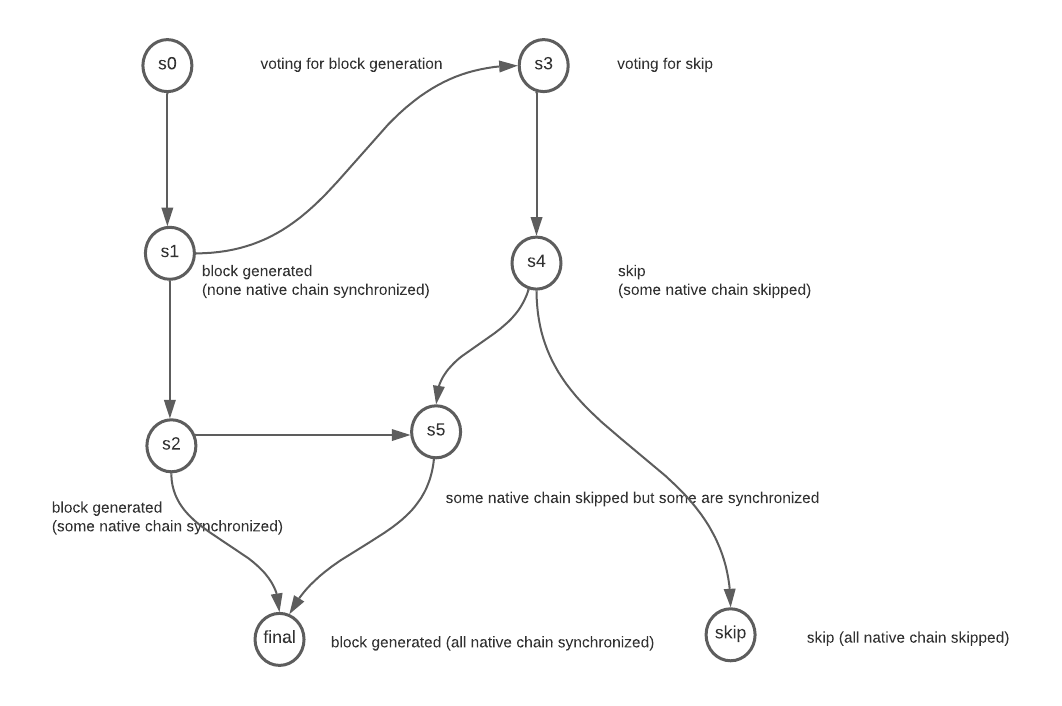
\includegraphics[scale=0.2]{state-transition.png}
\end{center}
\caption{State transition}
\label{state-transition}
\end{figure}

%then the voter needs to trigger another vote to skip the current round of block producing and send the skip signal to all native blockchains. Once all the native blockchains received the skip signal, they will not accept any block with the current round number and the next round of block generation can start. If one of the native blockchains received the synchronizing call of the generated block, then all the nodes need to perform a revoke-skip vote so that they can revoke the skip signal on native blockchains.

Notice that in the protocol, the interesting state is $s_4$ in which the block is generated and some nodes suspected that the finalizing stage is halted and vote for skip the current round. If any of the node notice that the block is partially finalized on a subset of native blockchains then it leads to $s_5$ and there is no need to skip. Otherwise the current round was skipped. Thus the final state of all native-block chains converges to the same state.

\subsection{Safety Property}
Recall that for a bundled transaction $tx = {tx_i}$. The safety property of a protocol to carry out $tx$ is that either all $tx_i$ succeed or none of them succeed.

Below we discuss the safety property of \dprotocol in three scenarios. First, we show that the safety property holds if a transaction $tx$ does not have an invoke transaction or any side effects. Second, we further prove that if all side-effects are safe then the safety property still holds. Finally, we show that if the first transaction of a bundled transaction $tx$ is an invoke transaction, then we can rely on our liveness property to ensure that if the invoke transaction succeeds then all following transactions will eventually be finalized.

%and if the invoke transaction fails then it can be revoked using a revoke transaction so that the global state stays the same. \\

\smallskip\noindent\emph{1. Bundled transaction with no invoke transaction}\\
If a bundled transaction does not start with an invoke transaction, then it means the bundled transaction is invoked directly on the aggregator chain. Because all components $tx_i$ of $tx$ are simulated and performed on the aggregator chain and a proof of the execution of $tx$ can not be generated if any $tx_i$ fails during the simulation, a transaction can only be executed as a whole. Once the ZKP proof was generated for the simulation, it will be used to convince each native chain to change its local state according to the result of the simulation.

%If the proof is valid and is submitted to native chains then it will pass the validation check and then we expect that the local state of the native chain will change accordingly with no exception.

%Since the liveness property promises that all native chains will eventually receive the valid proof, it remains to show that the state updating protocol in our proxy contract is safe.

%A smart contract is a piece of code that can not be changed once deployed, its behavior is fixed and predictable. Thus we can assume that our proxy contract always performs correctly according to its pre-defined functionality. Suppose that $s$ is the start global state, $tx$ is the transaction and $s'$ is the final state. When our proxy contract receives $MTH(s)$, $tx$, $MTH(s')$ and the state difference $\delta_{s}$ together with a zero-knowledge proof $p(MTH(s), MTH(s'), tx)$, our proxy contract will do the following:

%\begin{enumerate}[leftmargin=*]
%\item Proxy contract checks that pined local global hash equals $MTH(s)$. This makes sure that the current local state $s_i$ is consistent with the global state $s$.

%\item Proxy contract verifies the proof $p(s, s', tx)$. Once the verification succeeds, it can guarantee that $s'$ is a valid final state after simulating $tx$ over $s$.

%\item Compute the changes of $s_i$ and change the local state from $s_i$ to $(s_i)'$. Since updating the local state is a monadic function of the local state, it will never fail which means once the proof of $tx$ is verified, the local state will be changed correctly for sure.

%\item Proxy contract performs all the related side effects for each transactions $tx_k$ in bundled transaction $tx$. 
%\end{enumerate}

\smallskip\noindent\emph{2. Bundled Transaction with an Side-effects.}\\
We notice that side-effects is the only place where a finalizing call will fail even if the proof is correct. To address this problem, we break down side effects into two categories. The first category contains side effects like emit events, logging, or pure history recording which are naturally safe since it will never fail by design. The second category includes unsafe function calls like assets transfer. This kind of unsafe function can still be safe if we perform sanity checks in tx.

For example, if $tx_k$ in $tx$ will trigger a side-effect $e_k$ and $e_k$ is safe under condition $P$ where $P$ is a predicate of global state $s$, then we can insert a check after $tx_k$ as following:

\begin{code}
...
let s' = tx_k(s);
if !P_k(s'):
    raise Excepition(sainity check failure)
let s'' = tx_{k+1}(s);
...
\end{code}
Once $tx$ is modified so as above, a valid proof of a correct simulation of $tx$ will ensure not only the final state valid but all the sanity checks are all valid and $e_k$ will be safe for sure.\\

\noindent\smallskip\emph{3. Bundled Transaction with an Invoke Transaction.}\\
If a bundled transaction $tx$ starts with an invoke transaction $tx_0$ on $C_i$, then this invoke transaction on chain $C_i$ triggers the execution of the bundled transaction $tx$ by emitting an invoking event. This event is reported to the aggregator chain through a native chain ZK relayer.

%The aggregator chain bundled transaction simulator relies on the honesty of the reporter and if the relayer is hacked it can exploit the protocol by reporting malformed results of the invoke transaction. For example, in the transfer scenario, if a report reports the wrong amount of assets that have been transferred from Alice to Bob in Chain A then a successfully finalized $tx$ will trigger a wrong transfer from Bob to Alice on Chain B.

%To address this problem and make sure the protocol is safe even though the relayer is dishonest,
In this scenario, we split the process of the changes of global state $s$ into two stages. At first stage $s$ is changed to $s'$ after invoke transaction and at second stage $s'$ is changed to $s''$ after the whole simulation of $tx$.

During the first stage, $s'$ is pined in native chain $C_i$ once the invoke transaction is executed and the second stage is encoded by a zero-knowledge proof generated from \dprotocol node. During finalize, proof of $tx$ now encodes the proof from $s'$ to $s''$.

%To ensure that the invoke transaction $tx_0$ is reported correctly, the verifier only needs to compare the MTH of the local calculation of $s'$ and the hash provided by the aggregator chain Node. If the hash is the same, then it means $tx_0$ are reported honestly. Moreover since $s'$ are checked, $s''$ can be treated as a valid simulation from $s$ to $s''$. In conclusion, the finalization steps are listed as follows:

%\begin{enumerate}[leftmargin=*]
%\item Proxy contract checks that pined local global hash equals $MTH(s'')$. This makes sure that the current local state $s_k^i$ is consistent with the global state $s'$ after processing invoke transaction. Thus the invoke transaction are reported honestly.

%\item Proxy contract verifies the proof $p_{t}(s', s'', tx)$. Once the verification succeeds, it can guarantee that $s''$ is a valid final state after simulating $tx$ over $s$.

%\item Compute the changes of $(s^i)'$ and change the local state from $(s^i)'$ to $(s_i)''$. Since updating local state is a monadic function of the local state, it will never fail which means once the proof of $tx$ is verified, the local state will be changed correctly for sure.

%\item Proxy contract performs all the related side effects for each transactions $tx_k$ in bundled transaction $tx$. 
%\end{enumerate}

\subsection{Linearity Property}
In concurrent programming, an operation (or set of operations) is linearizable if it consists of an ordered list of invocation and response events. Since in each block generation round only one node wins the right to produce a block, the linearity hold iff and only if the final state simulated in the block can be represented as a sequence of bundled cross transactions $tx_i$. Since each block producer needs to create a zero-knowledge proof to show that $s' = tx_k \circ tx_{k-1} \circ \cdots tx_0(s)$, a valid proof already shows the linearity property. Thus in \dprotocol protocol, the linearity property holds trivially. 

\section{Implementation and Evaluation}
\label{chp:bench}
\subsection{Code base for \dprotocol}
We implemented the Aggregator chain based on substrate \cite{substrate}. Substrate is a blockchain development kit, with which users can customize a blockchain by combining rich blockchain building blocks. We start with a standard substrate setting and build our \dprotocol by providing our own consensus component, simulation component and finalizing component. As we described in Section \ref{consensus-stage}, the verifying process is done on native blockchains. Thus the main performance cost is spent on the ZKP part during consensus, simulation and proving stage. Since the ZKP performance is highly related to constraints size (CS) of ZKP circuits, below we will mainly use the number of constraints as a measurement of performance. 

\subsection {Consensus Component}
Recall that the consensus component needs to provide ZKP circuit for registering valid node, validating a registered node and voting the node to generate a new block. Also the voting process can be further splited into two parts: voter needs to generate and sending the voting ticket to target and winner needs to prove that he has received sufficient vote.  Thus the following four different circuits written in circom \cite{munoz2022circom} are needed for the consensus component (see Table \ref{tbl:consensus-cs}).

\begin{table}[!ht]
\small
\centering
\caption{Consensus Circuit Constraint Size}
\label{tbl:consensus-cs}
\begin{tabular}{ | c | c | c | c | c | }
\hline
Total Nodes & Circuit Name & Language & CS & Proofs \\
\hline
128 & register & circom & $2^{18}$ & 1\\
\hline
256 & register & circom & $2^{18}$ & 1\\
\hline
$2^{18}$ & register & circom & $2^{21}$ & 1\\
\hline
128 & node validation & circom & $2^{17}$ & 1\\
\hline
256 & node validation & circom & $2^{17}$ & 1\\
\hline
$2^{12}$ & node validation & circom & $2^{21}$ & 1 \\
\hline
128 & source voting & circom & $2^{17}$ & 1\\
\hline
256 & source voting & circom & $2^{17}$ & 1\\
\hline
$2^{12}$ & source voting & circom & $2^{17}$ & 1\\
\hline
128 & winner proving & circom & $2^{24}$ & 1\\
\hline
256 & winner proving & circom & $2^{24}$ & 2 \\
\hline
$2^{12}$ & winner proving & circom & $2^{24}$ & 16 \\
\hline
\end{tabular}
\end{table}
\begin{remark}
When winner proving that he has collected enough votes, he might need to provide more than one proof and each proves that certain amount of voter has voted him by sending him the voting proof.
\end{remark}

\subsection{Simulation Circuit}
Since the size of the simulation circuit usually depends on the transaction logic a user would like to execute, we provide an example to show the circuits size of building a multi-chain DEFI (decentralized finance \cite{zetzsche2020decentralized, chen2020blockchain}) system over ZK Multi-Blockchain Aggregator (see Table \ref{tbl:defi-cs}) using circom. In Table \ref{tbl:defi-cs} the AMM circuits denotes the multi-blockchain transactions of automated market maker \cite{mohan2022automated} and the state circuit denotes the circuit of Merkle tree manipulating interfaces. 

\begin{table}[h]
\small
\centering
\caption{DEFI Transaction Circuits}
\label{tbl:defi-cs}
\begin{tabular}{ | c | c | c | c | }
\hline
Number of $t_x$ & Circuit Name & Language & CS \\
\hline
8 & AMM circuit & Circom & $2^{14}$ \\
\hline
256 & AMM circuit & Circom & $2^{19}$ \\
\hline
8 & State circuit & Circom & $2^{16}$ \\
\hline
256 & State circuit & Circom & $2^{21}$ \\
\hline
\end{tabular}
\end{table}

\subsection{Proof Batching 
circuit}
The common way to batch multiple proofs into one single proof is to encode the plonk verify algorithm into ZKP circuits. Since the verify algorithm contains a lot of calculation of elliptic scalar multiplication, it is infeasible to implement such complex algorithm in Circom. Thus we encodes the algorithm using Halo2 \cite{halo2book} proving system (see Figure \ref{tbl:batch-proofs} for constraint size in Halo2).  

\begin{table}[!ht]
\small
\centering
\caption{Circuits for Batching Proofs}
\label{tbl:batch-proofs}
\begin{tabular}{ | c | c | c | c | }
\hline
Circuit Name & Language & CS \\
\hline
Elliptic curve scalar multiplication circuit & Halo2 & $7 \times 10^4$ \\
\hline
Transcript circuit & Halo2 & $2^{18}$ \\
\hline
Batch circuit & Halo2 & $2^{24}$ \\
\hline
\end{tabular}
\end{table}

\subsection{Evaluation Results}
The overall block generating time is the sum (some of the calculation can be executed in a concurrent manner) of the consensus stage, simulating stage, and proving stage. The time consuming of simulating stage is negligible, thus it is sufficient to calculate the time of consensus stage and proving stage. The average time consuming of $2^{20}$ constraints is about 6 sec using Rapidsnark on a 4 CPU computer with 128G memory. When batch proofs using Halo2 system, it takes 34 seconds more to batch the consensus proof with around 32 simulation proofs in a block on a 4 CPU computer with one NVIDIA GeForce RTX 3070 card. The overall performance of transaction handling is about 1 TPS(transaction per second) and can be scaled linearly if more hardware are provided.


\section{Related Works}
\label{chp:related-work}
\noindent
\emph{Notary Schemes.} The main idea of notary schemes is to elect one or more trusted nodes as a notary public and report transactions in different blockchain networks through notaries \cite{qin2018overview}. Therefore, all information transferred between different blockchains is completely managed by notaries. The centralized notary scheme has efficiency in procession events and simplicity in implementation. However, it suffers from the SPOF problem. Therefore, a multi-signature notary scheme may be proposed to reduce the trust in a certain centralized node. However, this multi-signature notary is surely non-permissionless and needs extra protocols to ensure liveness.

\smallskip\noindent\emph{SPV: Simplified Payment Verification.}
SPV \cite{lin2017survey,ray2020blwn} is a special case of one-directional state pining \cite{robinson2020merits}. In such protocols, the block header of $C_A$ and a Merkle proof of a particular transaction is monitored and sent to the target blockchain $C_B$. $C_B$ accepts the transaction by calculating the partial Merkle tree hash and compares it with the block header of $C_A$. The liveness property of this approach depends on the liveness of relayers of $C_A$ and the safety property relies on the block headers being reported to $C_B$ honestly. 
    
\smallskip\noindent\emph{Sidechains.}
The goal of sidechains \cite{singh2020sidechain} is to extend the scalability and functionality of the blockchain system. Sidechains can enforce the security of transactions on themselves by implementing a protocol that can be validated by consensus. Since the sidechain needs to update state changes back to the underlying blockchains, the blockchains need to trust or verify the transactions sent out by sidechains. The safety property again relies on whether observation of the source chain can be honestly reported to the side chain and whether the verifier on the target chain can reject all fraud transactions. In addition, since the sidechain can suffer from deny-of-service attacks that lead to non-finalization of a bundled transaction, the safety property also relies on the liveness property.

The liveness of sidechains relies on how robust the sidechain itself is and whether all the transactions that happened on the sidechain will get reported to the target chain eventually. Some improving ideas are given in Plasma \cite{poon2017plasma}.

\smallskip\noindent\emph{Cross Chain Gateway and Relayers.}
Cross Chain Gateway with relays is another extension of the idea of state pinning. While it enables blockchain interoperability applications including cross-chain token transfer, the safety property is attained at the cost of storing every single block header of the source blockchain \cite{belchior2021survey}. In general, the cost of storing such a state is very expensive.

\smallskip\noindent\emph{ZKBridge.}
A recent protocol, ZKBridge \cite{xie2022zkbridge-zkbridge}, proposed an efficient cross-chain bridge that guarantees strong security by using ZKP to provide trustless relayers. The trust base of ZKBridge requires that the light-client protocols of checking the blockhead of the source blockchain are secure. Compared with ZKBridge, our protocol is completely different in two aspects. First, we do not assume a secure light client but use a consensus algorithm to make sure the blockhead tracking process is permissionless. Second, ZKBridge still follows the traditional way of executing transactions on different blockchains and using relayers to synchronize them, so it does not scale well in the situation of a large number of involved blockchains since it needs to handle the interference between the blockchains in a case-by-case manner; instead, we simulate the transaction on our aggregator chain and convince native blockchains to update their local state by providing the ZKP of the simulation result, and hence provides a general solution to handle the interference. Thus, our protocol naturally has the linearizability property with no scalability problem when applied to scenarios with a large number of native blockchains.
%\newline
%In conclusion, we have the following (see Table: \ref{tab:related}).
%\begin{table*}[!h]
%\small
%\centering
%\caption{Related Work}\label{tab:related}
%\begin{tabular}{ | c | c | c | c | c |}
%\hline
%Protocol & Liveness & Trustless Safety & Permissionless & MultiChain Atomicity \\
%\hline
%NotarySchemes & yes & yes & no & no\\
%\hline
%SPV & yes & no & no & no \\
%\hline
%Peg & no & no & no & no\\
%\hline
%SideChain & yes & no & yes & yes\\ 
%\hline
%Gateway& yes & no & no & no\\ 
%\hline
%\end{tabular}
%\end{table*}


\bibliographystyle{plain}
\bibliography{main}


\end{document}

